% =====================================================================================
\section{Background and theory}
\label{sec:background}
% =====================================================================================

\subsection{From phases to a beam}
\label{sec:arraytheory}

For $N$ identical emitters at positions $x_n$ with pitch $d$, equal amplitudes and phases $\phi_n$, the far-field
intensity at angle $\theta$ from the surface normal is
\begin{equation}
  I(\theta) \;=\; \mathrm{EP}(\theta)\,\Bigl|\frac{1}{N}\sum_{n=1}^{N} \ee^{\,\ii(\phi_n - k_0 x_n \sin\theta)}\Bigr|^{2},
  \qquad k_0=\frac{2\pi}{\lambda},
  \label{eq:farfield}
\end{equation}
where $\mathrm{EP}(\theta)$ is the single-emitter (element) pattern and $\lambda$ the free-space wavelength.

\paragraph{Steering.} A linear ramp $\phi_n=n\,\Delta\phi$ points the beam at
\begin{equation}
  \sin\theta_0 \;=\; \frac{\Delta\phi\,\lambda}{2\pi d}
  \label{eq:steer}
\end{equation}
(\cref{fig:basics}a). Only the step between neighbours matters; a common offset changes nothing and is left free
throughout.

\paragraph{Field of view.} The pattern repeats when $\sin\theta$ shifts by $\lambda/d$, producing grating lobes. A
single beam is obtained for $|\Delta\phi|\le\pi$, that is,
\begin{equation}
  |\theta_0| \;\le\; \arcsin\frac{\lambda}{2d} \;=\; \ang{22.8}
  \qquad(\lambda=\qty{1.55}{\micro\metre},\ d=\qty{2}{\micro\metre}).
  \label{eq:fov}
\end{equation}
At this pitch the nearest grating lobe is only \qty{2.4}{\decibel} below the main beam. Every
\qty{2}{\micro\metre}-pitch array has this limitation, regardless of how the phases are set, so side-lobe
suppression cannot distinguish between designs. We therefore use the Strehl ratio (\cref{sec:metrics}) as the
measure of beam quality. The \qty{66}{\micro\metre} aperture gives a beam \ang{1.2} wide (FWHM), so the field holds
about \num{34} resolvable spots.

\paragraph{Focusing.} A parabolic phase with the centre leading the edges focuses the light to a line at
distance $f$ (\cref{fig:basics}b). In the paraxial limit
\begin{equation}
  \phi(x) \;=\; c - \frac{k_0 x^{2}}{2f},
  \qquad
  a \;\equiv\; \phi(0)-\phi(X) \;=\; \frac{k_0 X^{2}}{2f},
  \label{eq:lens}
\end{equation}
where $X=\qty{32}{\micro\metre}$ is the half-aperture and $a$ the \emph{lens strength}. For this array
$a\,f=\qty{2076}{\rad\,\micro\metre}$, so $a=\qty{1}{\rad}$ corresponds to $f=\qty{2.1}{\milli\metre}$.

\begin{figure}[htbp]
  \centering
  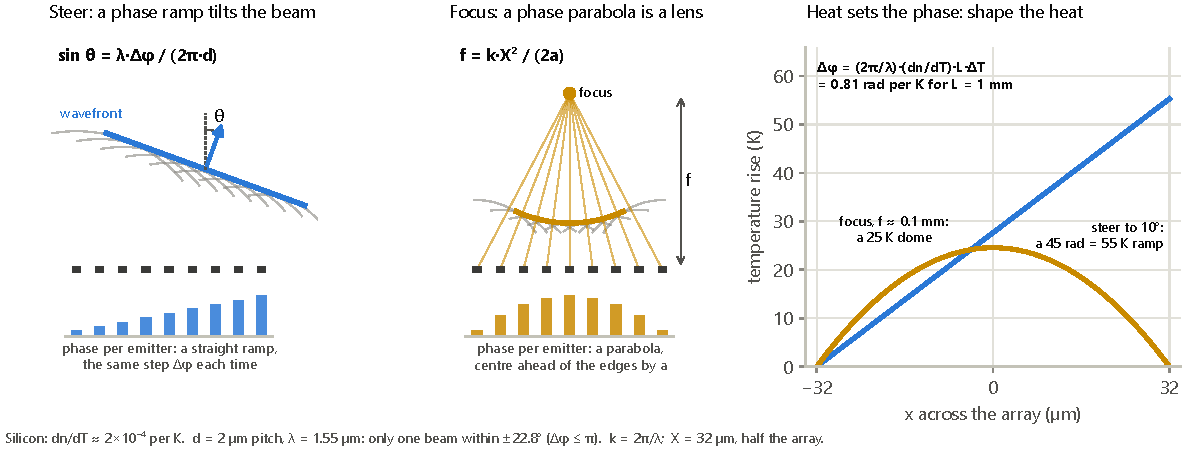
\includegraphics[width=\linewidth]{fig15_opa_basics}
  \caption{Steering and focusing (schematic, nine emitters). (a)~A linear phase ramp tilts the wavefront:
  $\sin\theta=\lambda\Delta\phi/(2\pi d)$. (b)~A parabolic phase focuses at $f=k_0X^2/(2a)$. (c)~The phase follows
  the temperature, \qty{0.81}{\rad\per\kelvin} for a \qty{1}{\milli\metre} heater, so the temperature must have the
  shape of the required phase. Shown: the \ang{10} ramp (\qty{45}{\rad}, \qty{55}{\kelvin} across the array) and a
  \qty{20}{\rad} lens.}
  \label{fig:basics}
\end{figure}

\subsection{From heat to phase}
\label{sec:heatphase}

A waveguide section of length $\Lh$ heated by $\Delta T$ delays its light by
\begin{equation}
  \phi \;=\; k_0\,\frac{\dd\neff}{\dd T}\,\Delta T\,\Lh ,
  \label{eq:phaseT}
\end{equation}
where $\neff$ is the effective index of the mode. For our waveguide $\dndT=\qty{2.009e-4}{\per\kelvin}$
(\cref{sec:modelA}), so a $2\pi$ shift needs \qty{7.7}{\kelvin\milli\metre}.

The heaters are much longer than the layer stack is thick, so temperature is computed in the cross-section, per
unit length. A heater at $\xh$ dissipating $P/\Lh$ per unit length raises the core at $x$ by
$\Delta T(x)=R(x;\xh)\,P/\Lh$, where $R$, the \emph{thermal kernel}, is in \unit{\KmW}. Substituting into
\cref{eq:phaseT}, the heater length cancels:
\begin{equation}
  \phi(x) \;=\; \gamma\,R(x;\xh)\,P,
  \qquad \gamma \equiv k_0\,\frac{\dd\neff}{\dd T} = \qty{814.4}{\rad\per\kelvin\per\metre}.
  \label{eq:phaseP}
\end{equation}
The phase depends only on total heater power. The length sets the temperature, $\Delta T=\phi/(\gamma\Lh)$, and
therefore enters only as a constraint. For the core under a heater, the power for a phase of $\pi$ is
\begin{equation}
  \Ppi \;=\; \frac{\pi}{\gamma\,R(\xh;\xh)} ,
  \label{eq:Ppi}
\end{equation}
so a lower $\Ppi$ requires a larger thermal resistance from the core to the heat sink. That resistance, together
with the heat capacity of the heated material, also sets the response time, so power and speed trade against each
other.

\subsection{Several heaters: superposition}
\label{sec:superposition}

For $K$ heaters at $x_k$ with powers $P_k$, the phase at emitter $n$ is taken as the sum of the single-heater
contributions,
\begin{equation}
  \phi_n \;=\; \sum_{k=1}^{K} G_{nk}\,P_k,
  \qquad
  G_{nk} \;=\; \gamma\,R(x_n;x_k),
  \label{eq:G}
\end{equation}
or $\bm\phi=G\bm P$. This step underlies every result in the report, so we justify it.

\paragraph{Proof.} Let $u=T-T_0$ be the temperature rise. With temperature-independent conductivity $k(\bm r)$,
the steady temperature satisfies
\begin{equation}
  \mathcal L u \;\equiv\; -\nabla\!\cdot\!\bigl(k\,\nabla u\bigr) \;=\; q(\bm r),
  \label{eq:heat}
\end{equation}
with $u=0$ on the substrate bottom and $\bm n\cdot k\nabla u=0$ on all other boundaries,
where $q=\sum_k q_k$ is the heat generated by all heaters. Let $u_k$ solve \cref{eq:heat} with heater $k$ alone.
The operator $\mathcal L$ is linear and both boundary conditions are homogeneous, so $u_\Sigma=\sum_k u_k$ satisfies
$\mathcal L u_\Sigma=\sum_k q_k=q$ and the same boundary conditions. The solution of \cref{eq:heat} is unique: if
$u_1$ and $u_2$ both solve it, their difference $w$ obeys $\mathcal Lw=0$ with the same homogeneous conditions, and
multiplying by $w$ and integrating by parts gives $\int k\,|\nabla w|^2\,\dd A=0$, so $w$ is constant and, since
$w=0$ on the substrate bottom, zero. Hence $u=\sum_k u_k$ exactly. Each $u_k$ scales linearly with $P_k$, and the
phase is linear in temperature (\cref{eq:phaseT}, confirmed to \qty{0.3}{\percent} by a coupled mode solve in
\cref{sec:comsolchecks}), which gives \cref{eq:G}. The same argument applies to the time-dependent equation, so
step responses also superpose.

\paragraph{Where it fails, and by how much.} Superposition requires $k$ independent of temperature. In reality
oxide conducts slightly better and silicon slightly worse when hot. The thermal model was therefore run with
temperature-dependent conductivities and two heaters \qty{6}{\micro\metre} apart, each alone and both together,
for both stacks (\cref{sec:modelF}). At peak rises of \qty{115}{\kelvin} (standard stack) and \qty{177}{\kelvin}
(undercut), the sum of the single-heater profiles exceeds the two-heater solution by \qty{1.7}{\percent} and
\qty{2.8}{\percent} of the peak. This discrepancy is fully explained by the temperature dependence: after the
Kirchhoff transform of \cref{sec:nonlinear}, the residual is \qty{0.08}{\percent} and \qty{0.14}{\percent}. Using
the same transform, the error of plain superposition for the slot design at \ang{10} with \qty{1}{\milli\metre}
heaters (peak \qty{63}{\kelvin}) is \qty{0.37}{\percent} of the peak (\qty{0.23}{\kelvin}). Superposition is
therefore exact for the linear model and accurate to better than \qty{0.5}{\percent} at the operating
temperatures used here; the residual temperature effect is treated in \cref{sec:nonlinear}.

\paragraph{Consequence.} Because heat conduction smooths its sources, $G$ can only produce phase profiles that are
smooth on the scale $\Lth$; for a kernel depending only on $x-\xh$ its singular values are the kernel's Fourier
transform. The simplest smooth steady states of a heated membrane are exactly the two profiles needed here: between
a heater and a heat sink with no losses, $u''=0$, a straight line (a ramp); for uniform heating between two sinks,
$u''=\text{const}$, a parabola (a lens). The designs of \cref{sec:steering,sec:lens} rely on this.

\subsection{Related work}
\label{sec:related}

\paragraph{Phase shifters.} Removing the heat path lowers $\Ppi$ from \qtyrange{20}{30}{\milli\watt} on a solid
stack~\cite{jacques2019} to about \qty{1}{\milli\watt} with an undercut~\cite{parsons2025} and
\qty{0.5}{\milli\watt} with suspended arms~\cite{fang2011}, at the cost of millisecond response. Folding the
waveguide through the heater several times reaches \qty{0.05}{\milli\watt}~\cite{lu2015}.

\paragraph{Steering with few signals.} Existing designs build the ramp from heater \emph{geometry}, giving each
waveguide a different heated length: a single triangular electrode~\cite{vanacoleyen2009}, identical shifters
cascaded along a feed bus~\cite{yaacobi2014,poulton2016}, and meandered heaters that also
focus~\cite{hosseini2025}. Few-heater tunable lenses have used shaped heaters on a slab
metalens~\cite{liu2023} and the same meanders~\cite{hosseini2025}.

\paragraph{Deliberate heat profiles.} We found no paper that sets a steering or lens profile across many
waveguides from the spreading of heat from a few heaters. The closest prior art is two patents that use
intentional thermal profiles to \emph{correct} an array, for aberrations~\cite{us10976542} and for crosstalk and
gradients~\cite{us10775559}. The present work differs in using spread heat as the actuator and in shaping
the membrane so that the profile is the one required. The literature search screened the papers citing
Refs.~\cite{vanacoleyen2009,yaacobi2014} and is not exhaustive.
